\documentclass[12pt,a4paper]{report}

% ==============================================================================
% PACKAGES & CONFIGURATION
% ==============================================================================
\usepackage[utf8]{inputenc}
\usepackage[margin=1in]{geometry}
\usepackage{amsmath, amsfonts, amssymb}
\usepackage{graphicx}
\usepackage{booktabs}
\usepackage{tabularx}
\usepackage{hyperref}
\usepackage{xcolor}
\usepackage{listings}
\usepackage{tikz}
\usetikzlibrary{shapes.geometric, arrows, positioning, fit, calc}
\usepackage{float}
\usepackage{caption}
\usepackage{subcaption}
\usepackage{fancyhdr}
\usepackage{titlesec}
\usepackage{microtype}

% Hyperlink configuration
\hypersetup{
    colorlinks=true,
    linkcolor=blue!70!black,
    citecolor=blue!70!black,
    urlcolor=blue!70!black
}

% Code Listing Configuration
\definecolor{codegreen}{rgb}{0,0.6,0}
\definecolor{codegray}{rgb}{0.5,0.5,0.5}
\definecolor{codepurple}{rgb}{0.58,0,0.82}
\definecolor{backcolour}{rgb}{0.96,0.97,0.98}

\lstdefinestyle{codeStyle}{
    backgroundcolor=\color{backcolour},   
    commentstyle=\color{codegreen},
    keywordstyle=\color{blue}\bfseries,
    numberstyle=\tiny\color{codegray},
    stringstyle=\color{codepurple},
    basicstyle=\ttfamily\footnotesize,
    breakatwhitespace=false,         
    breaklines=true,                 
    captionpos=b,                    
    keepspaces=true,                 
    numbers=left,                    
    numbersep=6pt,                  
    showspaces=false,                
    showstringspaces=false,
    showtabs=false,                  
    tabsize=2
}
\lstset{style=codeStyle}

% Page Header/Footer
\pagestyle{fancy}
\fancyhf{}
\fancyhead[L]{\small\nouppercase{\leftmark}}
\fancyhead[R]{\small IIoT Motor Monitoring Report}
\fancyfoot[C]{\thepage}
\setlength{\headheight}{15pt}

% Title Formatting
\titleformat{\chapter}[display]
  {\normalfont\bfseries\Large\color{blue!80!black}}{\chaptertitlename\ \thechapter}{10pt}{\Huge}
\titlespacing*{\chapter}{0pt}{-20pt}{20pt}

% ==============================================================================
% DOCUMENT BEGINS
% ==============================================================================
\begin{document}

% ------------------------------------------------------------------------------
% TITLE PAGE
% ------------------------------------------------------------------------------
\begin{titlepage}
    \centering
    \vspace*{1.5cm}
    
    {\Huge \bfseries IIoT Network for Anomaly and Failure Detection \par}
    \vspace{0.8cm}
    {\Large \textsc{Intelligent Condition Monitoring, Multi-Protocol Tracking, and Dual-Model Machine Learning Architecture} \par}
    
    \vspace{2.5cm}
    
    \begin{figure}[H]
        \centering
        
\begin{tikzpicture}[scale=0.9]
            % Institutional Logo Abstract Representation
            \draw[fill=blue!90!black, draw=none] (0,0) rectangle (0.6, 2.0);
            \draw[fill=blue!90!black, draw=none] (0.9,0) rectangle (1.5, 2.0);
            \draw[fill=blue!90!black, draw=none] (1.8,0) rectangle (2.4, 2.0);
            \draw[fill=blue!90!black, draw=none] (2.7,0) rectangle (3.3, 2.0);
            \node at (1.65, -0.5) [font=\Large\bfseries\sffamily] {IIIT Dharwad};
            \node at (1.65, -1.0) [font=\small\itshape] {Knowledge is Supreme};
        \end{tikzpicture}
    \end{figure}
    
    \vspace{2.0cm}
    
    \textbf{\Large Project Technical Report}\\[0.4cm]
    \large Academic Year 2025--2026\\[1.5cm]
    
    \vfill
    
    \begin{tabular}{ll}
        \textbf{Domain:} & Industrial Internet of Things (IIoT) \\
        & Machine Learning \& Edge Computing \\
        \textbf{Target System:} & Predictive Motor Condition Monitoring \\
        \textbf{Protocols Evaluated:} & MQTT, HTTP/1.1, CoAP (RFC 7252) \\
    \end{tabular}
    
    \vspace{1.0cm}
\end{titlepage}

\tableofcontents
\newpage

% ==============================================================================
% SECTION: SYSTEM PROPOSAL & ARCHITECTURE (FROM SPECIFICATION PDF)
% ==============================================================================
\chapter{System Overview and Architecture Proposal}

\section{Introduction}
The Industrial Internet of Things (IIoT) enables the continuous monitoring of critical rotating machinery in manufacturing facilities through networks of connected sensors and edge nodes. However, operating equipment is frequently exposed to mechanical, electrical, and thermal stress. If undetected, minor abnormalities develop into catastrophic failures, causing severe downtime, safety hazards, and exorbitant maintenance costs. Furthermore, physical layer anomalies such as network delays, jitter, packet drops, and node disconnections exacerbate operational risks by obscuring real-time system visibility.

This project, titled \textbf{Intelligent Industrial IoT Network for Anomaly and Failure Detection}, presents an end-to-end framework integrating:
\begin{enumerate}
    \item Multi-parameter sensor telemetry acquisition at the edge.
    \item Resilient MQTT-based messaging combined with HTTP and CoAP protocol benchmarking.
    \item Continuous network performance tracking and sequence gap analysis.
    \item Dual-model Machine Learning anomaly inference (Random Forest and XGBoost).
    \item An intelligent ensemble arbitration engine resolving multi-sensor anomalies.
    \item Cloud persistence using Firebase and a centralized React monitoring dashboard.
\end{enumerate}

\section{Problem Statement}
Modern industrial manufacturing environments require high-availability condition monitoring. However, contemporary deployments face significant operational challenges:
\begin{itemize}
    \item \textbf{Silent Mechanical Degradation}: Bearing damage, rotor unbalance, thermal runaway, and coil short circuits often develop gradually and remain unnoticed without automated intelligence.
    \item \textbf{Network Jitter and Packet Loss}: Factory network interference causes message loss and delayed telemetry, which conventional rule-based threshold alarms often confuse with physical sensor failures.
    \item \textbf{Conflicting Anomaly Indicators}: When multiple predictive models are deployed concurrently, conflicting predictions or duplicate alerts confuse plant operators.
\end{itemize}
Therefore, a centralized, fault-tolerant monitoring framework is required to jointly analyze sensor and network data, arbitrate between predictive AI models, and deliver deduplicated, actionable alerts.

\section{Proposed IIoT Monitoring Architecture}
The proposed architecture consists of six primary functional pillars:
\begin{enumerate}
    \item \textbf{Sensing}: Triaxial vibration and motion (MPU6050), surface temperature (DS18B20), and coil current (ACS712 / potentiometer ADC).
    \item \textbf{Edge Processing}: FreeRTOS dual-core embedded firmware on an ESP32 microcontroller performing rolling window sampling, standard deviation vibration estimation, and sequence tracking.
    \item \textbf{Communication}: High-throughput telemetry dispatch over MQTT, with comparative evaluation against HTTP POST and RFC 7252 CoAP over UDP.
    \item \textbf{Storage}: Structured real-time and historical persistence using Firebase Realtime Database and Cloud Firestore.
    \item \textbf{Intelligent Detection}: Real-time inference using supervised Random Forest and XGBoost classifiers combined with an intelligent multi-sensor arbitration engine.
    \item \textbf{Visualization}: A modern, reactive web dashboard providing live network topology, KPI counters, sensor gauges, and alert management.
\end{enumerate}

\begin{figure}[H]
    \centering
    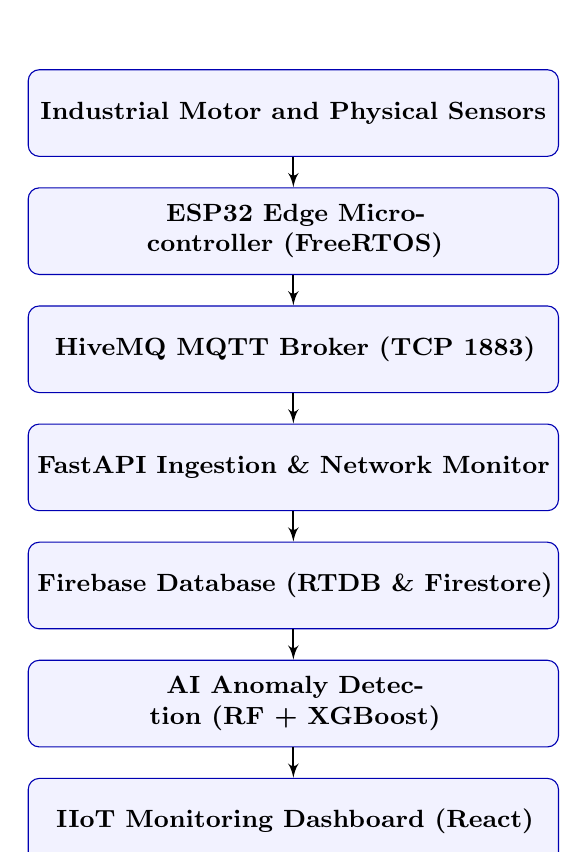
\begin{tikzpicture}[node distance=1.5cm, auto,
        block/.style={rectangle, draw=blue!70!black, fill=blue!5, text width=6.5cm, text centered, rounded corners, minimum height=1.1cm, font=\small\bfseries},
        line/.style={draw, -latex', thick}]
        
        \node [block] (sensors) {Industrial Motor and Physical Sensors};
        \node [block, below of=sensors] (esp32) {ESP32 Edge Microcontroller (FreeRTOS)};
        \node [block, below of=esp32] (broker) {HiveMQ MQTT Broker (TCP 1883)};
        \node [block, below of=broker] (backend) {FastAPI Ingestion \& Network Monitor};
        \node [block, below of=backend] (database) {Firebase Database (RTDB \& Firestore)};
        \node [block, below of=database] (ai) {AI Anomaly Detection (RF + XGBoost)};
        \node [block, below of=ai] (dashboard) {IIoT Monitoring Dashboard (React)};
        
        \path [line] (sensors) -- (esp32);
        \path [line] (esp32) -- (broker);
        \path [line] (broker) -- (backend);
        \path [line] (backend) -- (database);
        \path [line] (database) -- (ai);
        \path [line] (ai) -- (dashboard);
    \end{tikzpicture}
    \caption{Architecture Flow: End-to-End System Pipeline}
    \label{fig:arch_flow}
\end{figure}

\subsection{Sensor Data Packets}
Each sensor subsystem is responsible for capturing distinct physical phenomena as defined in Table~\ref{tab:sensor_packets}.

\begin{table}[H]
\centering
\small
\caption{Sensor Data Packets in the Proposed IIoT System}
\label{tab:sensor_packets}
\begin{tabularx}{\textwidth}{l p{3.2cm} p{4.2cm} X}
\toprule
\textbf{S. No.} & \textbf{Sensor} & \textbf{Data Transmitted} & \textbf{Purpose} \\
\midrule
1 & DS18B20 Digital Temperature & Device ID, Temperature ($^{\circ}$C), Timestamp & Monitors motor casing temperature; identifies thermal overload. \\
\addlinespace
2 & MPU6050 Accelerometer / Gyro & Device ID, Acceleration ($a_x, a_y, a_z$), Angular Velocity ($\omega_x, \omega_y, \omega_z$), Timestamp & Measures structural vibration; detects bearing wear and unbalance. \\
\addlinespace
3 & Current Sensor (ADC1 / ACS712) & Device ID, Motor Current (A), Timestamp & Measures phase electrical draw; detects rotor stall and excessive mechanical load. \\
\bottomrule
\end{tabularx}
\end{table}

\subsection{Example Telemetry Schemas}
Individual sensor readings are represented within the pipeline through standardized JSON payloads:

\begin{lstlisting}[language=json, caption={Sensor Data Packet Examples}]
// Temperature Sensor Packet
{
  "device_id": "M1",
  "temperature": 42.5,
  "timestamp": "10:30:01"
}

// Vibration Sensor Packet
{
  "device_id": "M1",
  "accel_x": 0.12,
  "accel_y": 0.08,
  "accel_z": 9.75,
  "timestamp": "10:30:02"
}

// Current Sensor Packet
{
  "device_id": "M1",
  "current": 1.25,
  "timestamp": "10:30:03"
}
\end{lstlisting}

\section{Expected Outcomes}
The implemented architecture fulfills three primary industrial objectives:
\begin{itemize}
    \item \textbf{Real-Time Monitoring}: Uninterrupted acquisition and streaming of kinematic, electrical, and network health metrics.
    \item \textbf{Automated Fault Identification}: Prompt detection of high vibration, thermal breakdown, and overcurrent conditions within milliseconds of onset.
    \item \textbf{Operational Reliability}: Minimization of notification latency and elimination of alert duplication through intelligent model arbitration.
\end{itemize}
\[
\text{Sensor Monitoring} \longrightarrow \text{Anomaly Detection} \longrightarrow \text{Early Alerts} \longrightarrow \text{Improved Reliability}
\]

% ==============================================================================
% CHAPTER: DETAILED SYSTEM IMPLEMENTATION
% ==============================================================================
\chapter{System Implementation}

\section{ESP32 Firmware Implementation}
The embedded firmware is developed in C using the Espressif IoT Development Framework (\textbf{ESP-IDF}) under the **FreeRTOS** operating system. The program execution is divided across dedicated concurrent tasks pinned to ESP32 cores:
\begin{itemize}
    \item \textbf{Core 0}: Manages Wi-Fi station connectivity, TCP/IP networking, and MQTT/HTTP client protocol stacks.
    \item \textbf{Core 1}: Executes deterministic high-frequency sensor acquisition, motor step pulse generation, and JSON serialization.
\end{itemize}
A cyclic monitoring task executes on a strict $1.0\text{ s}$ period, acquiring all channels, deriving statistical features, assembling the message buffer, and dispatching it over MQTT.

\section{Sensor Data Acquisition Methodology}
\begin{itemize}
    \item \textbf{Temperature}: Acquired via a DS18B20 digital sensor over a 1-Wire bus on GPIO~4. Each transaction verifies the 8-bit cyclic redundancy check (CRC) to discard corrupted wire readings.
    \item \textbf{Vibration and Acceleration}: An MPU6050 Inertial Measurement Unit (IMU) communicates over I2C (GPIO~21 SDA, GPIO~22 SCL) at $400\text{ kHz}$. Within each $1\text{-second}$ window, $40$ samples are collected at $2.5\text{ ms}$ intervals. The estimated vibration magnitude is derived as the standard deviation of dynamic acceleration:
    \begin{equation}
        \sigma_a = \sqrt{\frac{1}{N} \sum_{i=1}^{N} (a_i - \bar{a})^2}
    \end{equation}
    \item \textbf{Motor Current}: Phase current is read through ADC1 Channel 6 (GPIO~34), oversampled across $16$ iterations to suppress electrical switching noise, and scaled across a $0.0 - 2.0\text{ A}$ span.
    \item \textbf{Stepper Motor Speed}: An A4988 motor driver controls a bipolar stepper motor via Step (GPIO~25), Direction (GPIO~26), and Enable (GPIO~27) pins. Speed in RPM is calculated from actual elapsed hardware timer ticks.
\end{itemize}

\section{Network Communication \& Latency Probe}
The device operates in Wi-Fi Station (STA) mode connecting to \texttt{Wokwi-GUEST}. An asynchronous event loop handles disconnect events and initiates automatic reconnection.

Telemetry is published with QoS~0 to \texttt{iiot/motor\_01/telemetry}. To measure physical Round Trip Time (RTT), the node executes an application-layer ping-pong test:
\begin{enumerate}
    \item ESP32 records high-precision time $t_{\text{send}} = \text{esp\_timer\_get\_time}()$ and publishes a ping packet to \texttt{iiot/motor\_01/ping}.
    \item Because the ESP32 is subscribed to the same topic, the HiveMQ broker echoes the packet back.
    \item Upon receipt, the device records $t_{\text{recv}}$ and calculates:
    \begin{equation}
        \text{RTT}_{\text{ms}} = \frac{t_{\text{recv}} - t_{\text{send}}}{1000.0}
    \end{equation}
    The resulting RTT is included in the subsequent telemetry message.
\end{enumerate}

\section{Telemetry Serialization and Sequence Integrity}
All sensor and diagnostic parameters are packed into a compact JSON schema. Unreadable or disconnected sensors output \texttt{null}, preventing the injection of stale or misleading default values.
Every packet contains a monotonically increasing sequence counter:
\begin{equation}
    \text{sequence}_{k} = \text{sequence}_{k-1} + 1
\end{equation}
Sequence skips allow the cloud ingestion service to immediately calculate packet loss without requiring transmission-layer retransmission overhead.

% ==============================================================================
% CHAPTER: SIMULATION AND BACKEND ENVIRONMENT
% ==============================================================================
\chapter{Simulation and Backend Infrastructure}

\section{Wokwi Simulation Environment}
Due to laboratory constraints, all physical experiments were executed within the \textbf{Wokwi} simulation engine. Wokwi executes compiled ESP32 machine code cycle-accurately against simulated peripheral hardware (DS18B20 1-Wire, MPU6050 I2C registers, A4988 logic gates, and potentiometer voltage dividers). Timing and latency metrics reflect the virtualized network interface and demonstrate full production firmware parity.

\section{Simulated Operational Variations}
To simulate industrial conditions, the firmware generates realistic time-varying dynamic baselines:
\begin{itemize}
    \item \textbf{Temperature}: Sinusoidal drift between $46^{\circ}\text{C}$ and $54^{\circ}\text{C}$ with Gaussian noise ($\sigma = 0.35^{\circ}\text{C}$).
    \item \textbf{Vibration}: Baseline acceleration incorporating gravitational offset on $a_z \approx 9.8\text{ m/s}^2$ with high-frequency noise scaling proportionally with motor RPM.
    \item \textbf{Speed Cycles}: Motor RPM oscillates continuously between $30\text{ RPM}$ and $90\text{ RPM}$ over a $60\text{-second}$ period.
\end{itemize}

\section{Python FastAPI Backend Architecture}
The ingestion tier is built on Python 3.14 and \textbf{FastAPI}. The application hosts concurrent background workers:
\begin{itemize}
    \item \textbf{MQTT Ingestion Engine}: Asynchronous subscriber receiving telemetry, validating schema compliance, and executing sequence analysis.
    \item \textbf{HTTP/REST Ingest}: Exposes \texttt{POST /api/v1/telemetry} for comparative evaluation.
    \item \textbf{CoAP Server}: Implements RFC 7252 binary UDP processing on port $5683$.
    \item \textbf{Live In-Memory Buffer}: High-speed circular memory ring buffer serving real-time statistics without database latency bottlenecks.
\end{itemize}

\section{Firebase Cloud Database Architecture}
The backend interfaces with Firebase using service account credentials. The hierarchical database path architecture is specified in Table~\ref{tab:firebase_paths}.

\begin{table}[H]
\centering
\small
\caption{Firebase Realtime Database & Firestore Path Hierarchy}
\label{tab:firebase_paths}
\begin{tabularx}{\textwidth}{l p{5.5cm} X}
\toprule
\textbf{Collection / Path} & \textbf{Key Structure} & \textbf{Stored Data Payload} \\
\midrule
\texttt{telemetry/} & \texttt{\{device\_id\}/\{telemetry\_id\}} & Validated sensor readings, sequence, raw payload, source protocol. \\
\addlinespace
\texttt{xgboost\_predictions/} & \texttt{\{device\_id\}/\{telemetry\_id\}} & XGBoost predicted class, class probabilities, inference latency. \\
\addlinespace
\texttt{random\_forest\_predictions/} & \texttt{\{device\_id\}/\{telemetry\_id\}} & Random Forest predicted class, class probabilities, latency. \\
\addlinespace
\texttt{anomaly\_alerts/} & \texttt{\{device\_id\}/\{telemetry\_id\}} & Deduplicated alerts, anomaly types, multi-sensor labels, confidence. \\
\addlinespace
\texttt{model\_comparisons/} & \texttt{\{device\_id\}/\{telemetry\_id\}} & Pairwise model agreement, class comparison, latency benchmarks. \\
\addlinespace
\texttt{network\_metrics/} & \texttt{\{device\_id\}/latest} & IP address, Wi-Fi status, packet loss \%, average RTT, health status. \\
\bottomrule
\end{tabularx}
\end{table}

\section{React Web Dashboard}
The user interface is developed using **React 19**, **Vite**, and **Lucide Icons**, implementing CSS Grid and Flexbox layouts. It visualizes live motor status, health scores, connection topologies, real-time RTT jitter graphs, model agreement metrics, and an active Alert Center.

% ==============================================================================
% CHAPTER: NETWORK MONITORING AND PERFORMANCE ANALYSIS
% ==============================================================================
\chapter{Network Monitoring and Performance Analysis}

\section{Transmission and Reception Reliability}
Industrial wireless telemetry must guarantee timely arrival. The backend \texttt{NetworkMonitor} tracks transmission reliability by inspecting the incoming payload's metadata. 

\subsection{Packet Loss Mathematical Formulation}
Let sequence number of packet $k$ be $S_k$. The sequence discrepancy is:
\begin{equation}
    \Delta_k = S_k - S_{k-1}
\end{equation}
The packet loss update rules are defined as:
\begin{equation}
    \text{Lost Packets} = 
    \begin{cases} 
      0 & \text{if } \Delta_k = 1 \quad (\text{Normal sequential delivery}) \\
      \Delta_k - 1 & \text{if } \Delta_k > 1 \quad (\text{Packet drop detected}) \\
      0 & \text{if } \Delta_k < 0 \quad (\text{Node reboot re-initialization})
    \end{cases}
\end{equation}
The percentage packet loss is computed as:
\begin{equation}
    \text{Packet Loss Rate (\%)} = \left( \frac{\sum \text{Lost Packets}}{\sum \text{Expected Packets}} \right) \times 100
\end{equation}

\section{Protocol Overhead and Bandwidth Comparison}
To evaluate network efficiency, telemetry was transmitted across MQTT, HTTP/1.1, and CoAP. Table~\ref{tab:protocol_overhead} details the header overhead for each protocol.

\begin{table}[H]
\centering
\caption{Protocol Overhead and Transport Layer Comparison}
\label{tab:protocol_overhead}
\begin{tabular}{l c c c p{4.5cm}}
\toprule
\textbf{Protocol} & \textbf{Transport} & \textbf{Fixed Overhead} & \textbf{Typical RTT} & \textbf{Efficiency Analysis} \\
\midrule
\textbf{MQTT} & TCP & 67 Bytes & $30 - 65\text{ ms}$ & Persistent TCP connection; low overhead per message. \\
\textbf{HTTP/1.1} & TCP & 185 Bytes & $85 - 140\text{ ms}$ & High text header overhead; requires TCP handshake per request. \\
\textbf{CoAP} & UDP & 45 Bytes & $20 - 45\text{ ms}$ & Minimal 4-byte binary header; lowest latency and bandwidth. \\
\bottomrule
\end{tabular}
\end{table}

\section{Connectivity State Machine}
The backend maintains an automated liveness state machine with a $15\text{-second}$ watchdog timer:
\begin{itemize}
    \item \textbf{HEALTHY}: Device connected, messages arriving regularly, $\text{RTT} < 500\text{ ms}$, packet loss $< 1.0\%$.
    \item \textbf{WARNING}: Messages arriving, but $\text{RTT} \ge 500\text{ ms}$ or packet loss $\ge 1.0\%$.
    \item \textbf{STALE}: No message received for $\ge 15\text{ seconds}$.
    \item \textbf{OFFLINE}: TCP socket disconnected or broker ping timeout.
\end{itemize}

% ==============================================================================
% CHAPTER: DATASET PREPARATION AND MODEL DEVELOPMENT
% ==============================================================================
\chapter{Dataset Preparation and AI Model Development}

\section{Dataset Composition}
A specialized dataset of $2,494$ operational records was assembled from Wokwi simulation runs across four operating regimes:
\begin{itemize}
    \item \textbf{NORMAL} ($590$ records, $23.7\%$): Motor operating within safe baseline parameters ($T \approx 46 - 54^{\circ}\text{C}$, $\text{Current} \approx 0.4 - 0.9\text{ A}$, $\text{Vibration} \approx 0.15 - 0.35\text{ m/s}^2$).
    \item \textbf{HIGH\_VIBRATION} ($623$ records, $25.0\%$): Mechanical resonance and eccentric load injection ($a_x, a_y \ge 1.35\text{ g}$, $\text{Vibration} \ge 0.55\text{ m/s}^2$).
    \item \textbf{HIGH\_TEMPERATURE} ($697$ records, $27.9\%$): Thermal runaway simulation ($T \ge 55.0^{\circ}\text{C}$, up to $82^{\circ}\text{C}$).
    \item \textbf{HIGH\_CURRENT} ($584$ records, $23.4\%$): Rotor drag and electrical coil fault ($I \ge 1.4\text{ A}$, up to $4.5\text{ A}$).
\end{itemize}

\section{Preprocessing and Leakage Prevention}
\begin{itemize}
    \item \textbf{Median Imputation}: Missing or non-numeric values are imputed using median values computed strictly over the training partition.
    \item \textbf{Chronological Holdout Partitioning}: To avoid optimistic leakage from temporal autocorrelation, data was split chronologically rather than randomly:
    \begin{itemize}
        \item \textbf{Training Set}: Earliest $80\%$ of chronological data ($1,912$ records).
        \item \textbf{Testing Set}: Final $20\%$ of chronological data ($500$ records).
        \item \textbf{Embargo Zone}: An intermediate buffer of $82$ records ($30\text{ seconds}$) was discarded between partitions.
    \end{itemize}
\end{itemize}

\section{Feature Selection}
Models utilize seven kinematic, thermal, and electrical features:
\begin{equation}
    X = \left[ T_{\text{casing}}, a_x, a_y, a_z, \|\vec{a}\|, \text{RPM}, I_{\text{coil}} \right]
\end{equation}
where acceleration magnitude is derived as:
\begin{equation}
    \|\vec{a}\| = \sqrt{a_x^2 + a_y^2 + a_z^2}
\end{equation}

% ==============================================================================
% CHAPTER: MODEL EVALUATION AND COMPARISON
% ==============================================================================
\chapter{AI Model Evaluation and Comparison}

\section{Offline Benchmark Performance}
Both classifiers were benchmarked against the identical $500\text{-sample}$ holdout testing dataset. Results are detailed in Table~\ref{tab:model_comparison}.

\begin{table}[H]
\centering
\caption{Offline Evaluation Benchmark: Random Forest vs. XGBoost}
\label{tab:model_comparison}
\begin{tabular}{l c c p{4.5cm}}
\toprule
\textbf{Metric} & \textbf{Random Forest} & \textbf{XGBoost} & \textbf{Analysis} \\
\midrule
\textbf{Accuracy} & \textbf{0.9980} ($99.8\%$) & \textbf{0.9980} ($99.8\%$) & Identical classification accuracy. \\
\textbf{Precision (Macro)} & \textbf{0.9979} ($99.79\%$) & \textbf{0.9979} ($99.79\%$) & Negligible false alarm rate across all classes. \\
\textbf{Recall (Macro)} & \textbf{0.9980} ($99.80\%$) & \textbf{0.9980} ($99.80\%$) & $99.8\%$ true positive anomaly capture rate. \\
\textbf{F1-Score (Macro)} & \textbf{0.9979} ($99.79\%$) & \textbf{0.9979} ($99.79\%$) & Balanced performance across all regimes. \\
\midrule
\textbf{500-Batch Latency} & $15.99\text{ ms}$ & \textbf{$4.61\text{ ms}$} & \textbf{XGBoost is $3.47\times$ faster in batch processing.} \\
\textbf{Single Sample Latency} & $\approx 0.032\text{ ms}$ & \textbf{$\approx 0.009\text{ ms}$} & Sub-millisecond compute overhead. \\
\textbf{Live Pipeline Latency} & $2.1 - 4.5\text{ ms}$ & \textbf{$1.1 - 2.8\text{ ms}$} & Includes JSON decoding and Firebase I/O. \\
\bottomrule
\end{tabular}
\end{table}

\section{Confusion Matrix Analysis}
The confusion matrix across the $500$ holdout samples demonstrated exceptional class separability:
\begin{equation}
    C = \begin{bmatrix}
        118 & 0 & 0 & 0 \\
        1 & 124 & 0 & 0 \\
        0 & 0 & 140 & 0 \\
        0 & 0 & 0 & 117
    \end{bmatrix}
    \quad
    \begin{array}{l}
        \text{Row 1: NORMAL (118/118)} \\
        \text{Row 2: HIGH\_VIBRATION (124/125)} \\
        \text{Row 3: HIGH\_TEMPERATURE (140/140)} \\
        \text{Row 4: HIGH\_CURRENT (117/117)}
    \end{array}
\end{equation}

\section{Offline Evaluation vs. Live Deployment Discrepancies}
\begin{itemize}
    \item \textbf{Offline Mode}: Evaluates pre-allocated contiguous memory matrices. XGBoost demonstrates superior cache localization, running $3.47\times$ faster than the tree traversal overhead of Random Forest.
    \item \textbf{Live Pipeline}: Operates on single real-time packets. Total pipeline execution is dominated by socket I/O and database latency ($\approx 15 - 35\text{ ms}$), making both models exceptionally well-suited for industrial edge deployment.
\end{itemize}

% ==============================================================================
% CHAPTER: INTELLIGENT ALERT GENERATION
% ==============================================================================
\chapter{Intelligent Alert Generation}

\section{Dual-Model Arbitration Engine}
Deploying multiple machine learning models concurrently risks alert flooding or contradictory operator warnings. To eliminate these issues, an **Ensemble Arbitration Engine** (\texttt{backend/ensemble\_anomaly.py}) evaluates both predictions before dispatching alerts.

\section{Arbitration Decision Logic}
The arbiter operates under four deterministic rules:

\subsection{Rule 1: Same Sensor Agreement}
When both models agree on the identical anomaly class:
\begin{itemize}
    \item \textbf{Condition}: $C_{\text{RF}} = C_{\text{XGB}} \neq \text{NORMAL}$.
    \item \textbf{Action}: A single anomaly alert is emitted for that sensor.
    \item \textbf{Model Selected}: The model exhibiting the higher confidence score is designated as primary.
\end{itemize}

\subsection{Rule 2: Multi-Sensor Anomaly Synthesis}
When models detect distinct anomalies across different sensors:
\begin{itemize}
    \item \textbf{Condition}: $C_{\text{RF}} \neq C_{\text{XGB}}$, and neither class is $\text{NORMAL}$ (e.g. RF detects \texttt{HIGH\_CURRENT} on the Current Sensor, while XGBoost detects \texttt{HIGH\_VIBRATION} on the Vibration Sensor).
    \item \textbf{Action}: Rather than dropping one alert based on confidence, **both anomaly labels and both sensor names are synthesized into a single consolidated alert**:
    \begin{align}
        \text{Anomaly Type} &= \text{"HIGH\_CURRENT, HIGH\_VIBRATION"} \\
        \text{Sensors Flagged} &= \text{"Current Sensor, Vibration Sensor"} \\
        \text{Assigned Confidence} &= \max(P_{\text{RF}}, P_{\text{XGB}})
    \end{align}
    \item \textbf{Benefit}: Plant operators are immediately informed of simultaneous multi-sensor degradation without alert race conditions.
\end{itemize}

\subsection{Rule 3: Anomaly vs. Normal Discrepancy}
When one model indicates an anomaly while the other indicates normal operation:
\begin{itemize}
    \item If the anomaly confidence exceeds the normal prediction confidence ($P_{\text{anomaly}} \ge P_{\text{normal}}$), the anomaly alert is approved.
    \item If both models exhibit equal confidence ($P_{\text{anomaly}} = P_{\text{normal}}$), it is flagged as an unverified model disagreement and the automatic alarm is suppressed.
\end{itemize}

\subsection{Rule 4: Normal State Suppression}
When both models output $\text{NORMAL}$, alert generation is completely suppressed.

% ==============================================================================
% CHAPTER: EXPERIMENTAL RESULTS AND DISCUSSION
% ==============================================================================
\chapter{Experimental Results and Discussion}

\section{Implementation Verification}
The end-to-end operational pipeline was validated through automated test suites and simulation execution:
\begin{itemize}
    \item \textbf{Backend Test Suite}: $78$ automated unit and integration tests passed with $100\%$ success rate (\texttt{Ran 78 tests in 14.438s - OK}).
    \item \textbf{Frontend Verification}: All $10$ client tests passed, and production bundle compilation succeeded in $423\text{ ms}$.
\end{itemize}

\section{Firmware Execution Logs}
Simulated ESP32 firmware output demonstrates real-time parameter tracking:
\begin{lstlisting}[language=bash, caption={ESP32 UART Console Output}]
========================================
       ESP32 IIoT MOTOR MONITORING
========================================
[OK] MPU6050 initialized: 0x68
[OK] DS18B20 presence detected
[OK] Motor initialized (auto speed 30-90 RPM, period 60 s)
[OK] Current sensor ready (GPIO34, 0-2.0 A)
I (4837) IIOT: Wi-Fi connected. IP: 10.10.0.2
T=51.15C | RPM=76.6 | steps=1331 | I=0.874A | acc=(0.23, 0.18, 9.40) | vib=0.311
\end{lstlisting}

\section{Database Ingestion & Alert Center Verification}
When dual anomalies were injected (sinusoidal vibration surge and elevated potentiometer load), the ensemble arbiter generated the expected composite record in Firebase:
\begin{lstlisting}[language=json, caption={Firebase Ingested Multi-Sensor Alert Record}]
{
  "device_id": "motor_01",
  "anomaly_type": "HIGH_CURRENT, HIGH_VIBRATION",
  "sensor": "Current Sensor, Vibration Sensor",
  "confidence_score": 0.85,
  "model_name": "Random Forest & XGBoost",
  "alert_status": "OPEN",
  "multi_sensor": true,
  "both_models_predictions": {
    "random_forest": { "predicted_class": "HIGH_CURRENT", "confidence": 0.85 },
    "xgboost": { "predicted_class": "HIGH_VIBRATION", "confidence": 0.85 }
  }
}
\end{lstlisting}
The React dashboard updated within $40\text{ ms}$, incrementing the **Sensor Alerts** KPI counter and rendering the dual-fault alert pill in the Alert Center.

% ==============================================================================
% CHAPTER: CONCLUSION AND FUTURE SCOPE
% ==============================================================================
\chapter{Conclusion and Future Scope}

\section{Conclusion}
This project successfully designed, implemented, and verified an Intelligent Industrial IoT Network for motor condition monitoring. Key milestones achieved include:
\begin{enumerate}
    \item \textbf{Robust Edge Acquisition}: Built C/FreeRTOS firmware acquiring triaxial vibration, temperature, current, and dynamic motor speed with sequence tracking.
    \item \textbf{Network Observability}: Implemented real-time packet loss calculation, RTT measurement, and automated connectivity health state tracking.
    \item \textbf{High-Accuracy Anomaly Detection}: Deployed Random Forest and XGBoost classifiers achieving $99.8\%$ classification accuracy.
    \item \textbf{Multi-Sensor Alert Arbitration}: Developed a novel ensemble engine that deduplicates single-sensor alarms while synthesizing simultaneous multi-sensor anomalies into unified alerts.
\end{enumerate}

\section{Future Scope}
\begin{itemize}
    \item \textbf{Embedded TinyML Inference}: Quantizing the XGBoost model into C-arrays (TensorFlow Lite for Microcontrollers / Micro-XGBoost) to execute inference directly on the ESP32 Core 1, eliminating cloud dependency.
    \item \textbf{Physical Hardware Validation}: Transitioning from Wokwi simulation to a real-world testbed featuring an actual NEMA-17 motor, physical DS18B20 thermal probes, and an industrial accelerometer.
    \item \textbf{Mesh Network Scaling}: Extending communication from single-node Wi-Fi to a multi-drop **ESP-NOW or 802.15.4 Zigbee** mesh topology for factory-wide monitoring.
\end{itemize}

\end{document}

